\documentclass[10pt]{article}

\usepackage{graphicx}
\usepackage{amsmath}
%\usepackage[ansinew]{inputenc}
\usepackage[utf8]{inputenc}
\usepackage[spanish]{babel}
\usepackage{babelbib}
\usepackage[T1]{fontenc}
\usepackage[vmargin=4cm,hmargin=4cm,letterpaper]{geometry}
\usepackage{color}
\usepackage{framed}
\usepackage{hyperref}
\usepackage{natbib}

\usepackage{listings}
\definecolor{red}{RGB}{219,0,0}
\definecolor{pink}{RGB}{255,100,100}
\definecolor{gray}{RGB}{100,100,100}
\lstset{
		basicstyle=\tiny,
		frame=single,
		keywordstyle=\color{red},
		commentstyle=\color{gray},
		stringstyle=\color{pink},
		tabsize=3,
		language=verilog,
		backgroundcolor=\color{white}}

\usepackage{fancyhdr} 
\pagestyle{fancy}
\usepackage{lastpage}
\lhead{Laboratorio 3}
\chead{}
\rhead{Bitácora}
\lfoot{}
\cfoot{}
\rfoot{\footnotesize Page \thepage\ of \pageref{LastPage}}

\renewcommand{\headrulewidth}{0.4pt} 
\renewcommand{\footrulewidth}{0.4pt} 

\graphicspath{{images/}}	%%multimedia path
\setlength{\parindent}{0pt}
%%*************************************************************************
\begin{document}

\begin{huge}
\begin{center}
\textbf{Proyecto : Snake World y Controlador VGA}
\end{center}
\end{huge}

\begin{Large}
\begin{center}
Jose Apú (B10407), Francisco Molina (B14194), \\Marco Montero (A94000), Dennis Vargas (B16831)
\end{center}
\end{Large}

\section{Objetivo General}

Desarrollar el famoso juego de snake y un controlador VGA utilizando una FPGA.\\[0.3 cm] \cite{papilio}

\subsection{Objetivos específicos}
\begin{itemize}
\item Utilizar los periféricos de la tarjeta de desarrollo.
\item 
\item 
\end{itemize}

%%**********************************************************************
\section{Implementación}

La implementación se puede separar en: el controlador VGA, el módulo que controla el mundo y el que controla a la serpiente.
%%**************************************************
\subsection{Controlador VGA}

Lo primero consistión es desarrollar el controlador VGA. Este módulo se encarga de poder desplegar datos en una pantalla. Se realizó para una configuración de 640x480, para estó se tomaron los valores de la Figura \ref{vga-data}.\\

\begin{figure}[hbtp]
\centering
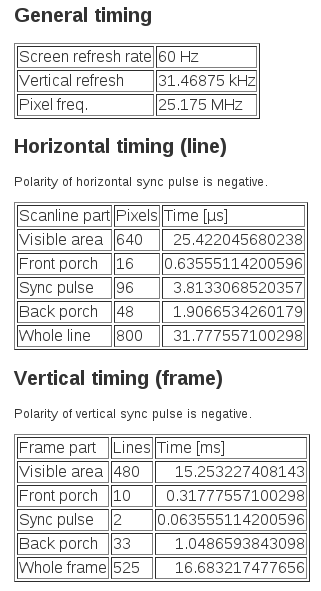
\includegraphics[width=0.4\textwidth]{vga-data.png}
\caption{VGA Signal 640 x 480 @ 60 Hz Industry standard timing}
\label{vga-data}
\end{figure}

Para este controlador lo importante es definír cuando HSYNC y cuando VSYNC se pone en 0 y cuando no. Para hay que tomar encuenta el diagrama de la Figura \ref{vga-pulse}.\\

\begin{figure}[hbtp]
\centering
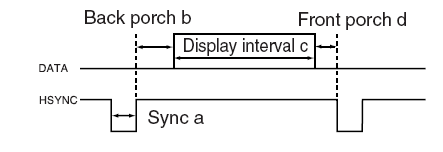
\includegraphics[width=0.4\textwidth]{vga-pulse.png}
\caption{Esquema de control}
\label{vga-pulse}
\end{figure}

Es necesario tener dos contadores, uno para las filas y otro para las columnas. Cuando llegue a un determinado valor cambia el valor de los SYNCs a cero. Además es necesario restaurarlos con valor inicial cero. Esta lógica se puede observar en el siguiente código:\\

\begin{lstlisting}
assign rowReset = (wRtemp == (WholeVFrame-1))? 1'b1:1'b0;
assign colReset = (wCtemp == (WholeHLine-1))? 1'b1:1'b0;

assign oVgaVsync = (wRtemp >= (VisibleVArea + FrontVPorch) && 
wRtemp <= (VisibleVArea + FrontVPorch + SyncVPulse))? 0:1;
assign oVgaHsync = (wCtemp >= (VisibleHArea + FrontHPorch) && 
wCtemp <= (VisibleHArea + FrontHPorch + SyncHPulse))? 0:1;
\end{lstlisting}




%%**************************************************
\subsection{El mundo}

Este módulo define el área de juego, así como la comida que va apareciendo de manera aleatoria. Si bien crear datos aleatorios no es algo trivial, podríamos hablar de generar datos seudoaleatorios. Para esto se utilizó el siguiente código:

\begin{lstlisting}
always @(iPixelRow,iPixelCol) 
begin		
	rLocationXTemp = ((x + 4271)*4273 - 9973*3)*57;
	rLocationYTemp = ((y + 3343)*3347 - 9857*3)*55;
	x = rLocationXTemp;
	y = rLocationYTemp;
end
\end{lstlisting}

$X$ y $Y$ toman un valor inicial e irá cambiando indefinidamente con la ecuación anterior. Con estos dos valores de elegi dónde irá la próxima comida cuando se necesite colocar nuevo comida (cada vez que la serpiente se come la comida). Los valores de rLocationXTemp, rLocationYTemp, x, y son número de 8 bits, por lo que nunca será más grande que 256 (el mundo es de 256x256).\\

Entonces para colocar la comida se utiliza el siguiente código (192 y 112 es para centrarlo al área de juego):

\begin{lstlisting}
begin
		oFoodLocationX = rLocationXTemp + 11'd192;
		oFoodLocationY = rLocationYTemp + 11'd112;
end
\end{lstlisting}

%%**************************************************
\subsection{La serpiente}

Este modulo se divide en tres módulos. El primero que genera la serpiente, otro que controla el movimiento y el otro que une estos dos módulos.

\subsubsection{SnakeIcon}

La serpiente se forma por un arreglo de cuadros (pixeles). En un inicio cuenta con 25 cuadros y puede llegar a un máximo de 100.\\

Cuando la serpiente se come una comida, el cuadro nuevo adopta el valor del cuadro anterior. Por ejemplo si tengo 30 cuadros, y como comida el cuadro 31 para a ser el cuadro 30, el 30 pasa hacer 29 hasta llegar al cuadro cero que toma e valor de la comida.\\

Este módulo también se encarga de verificar si uno pierde la partida, ya sea si se tocó así mismo o toco una pared.

\begin{lstlisting}
//Cuando toca una pared
		if (oSnakeLenght >= 8'd26 || iLocationX <= 11'd192 ||  
		                             iLocationX >= 11'd449 || 
		                             iLocationY <= 11'd112 || 
		                             iLocationY >= 11'd368)
			oGameOver = 1;
		else
			oGameOver = 0;

//Cuando se come asi mismo			
		for(j=100;j>=2;j=j-1) 
		begin
			//revisa si la cabeza tiene un valor igual a alguno del cuerpo 
			if(rBodyStack[0] == rBodyStack[j] && j <= oSnakeLenght)
				oGameOver = 1;
			else
				oGameOver = oGameOver;
		end	
\end{lstlisting}
		 
\subsubsection{SnakeMovement}


\subsubsection{SnakeMain}


%%**********************************************************************
\section{Resultados}

\begin{figure}[hbtp]
\centering
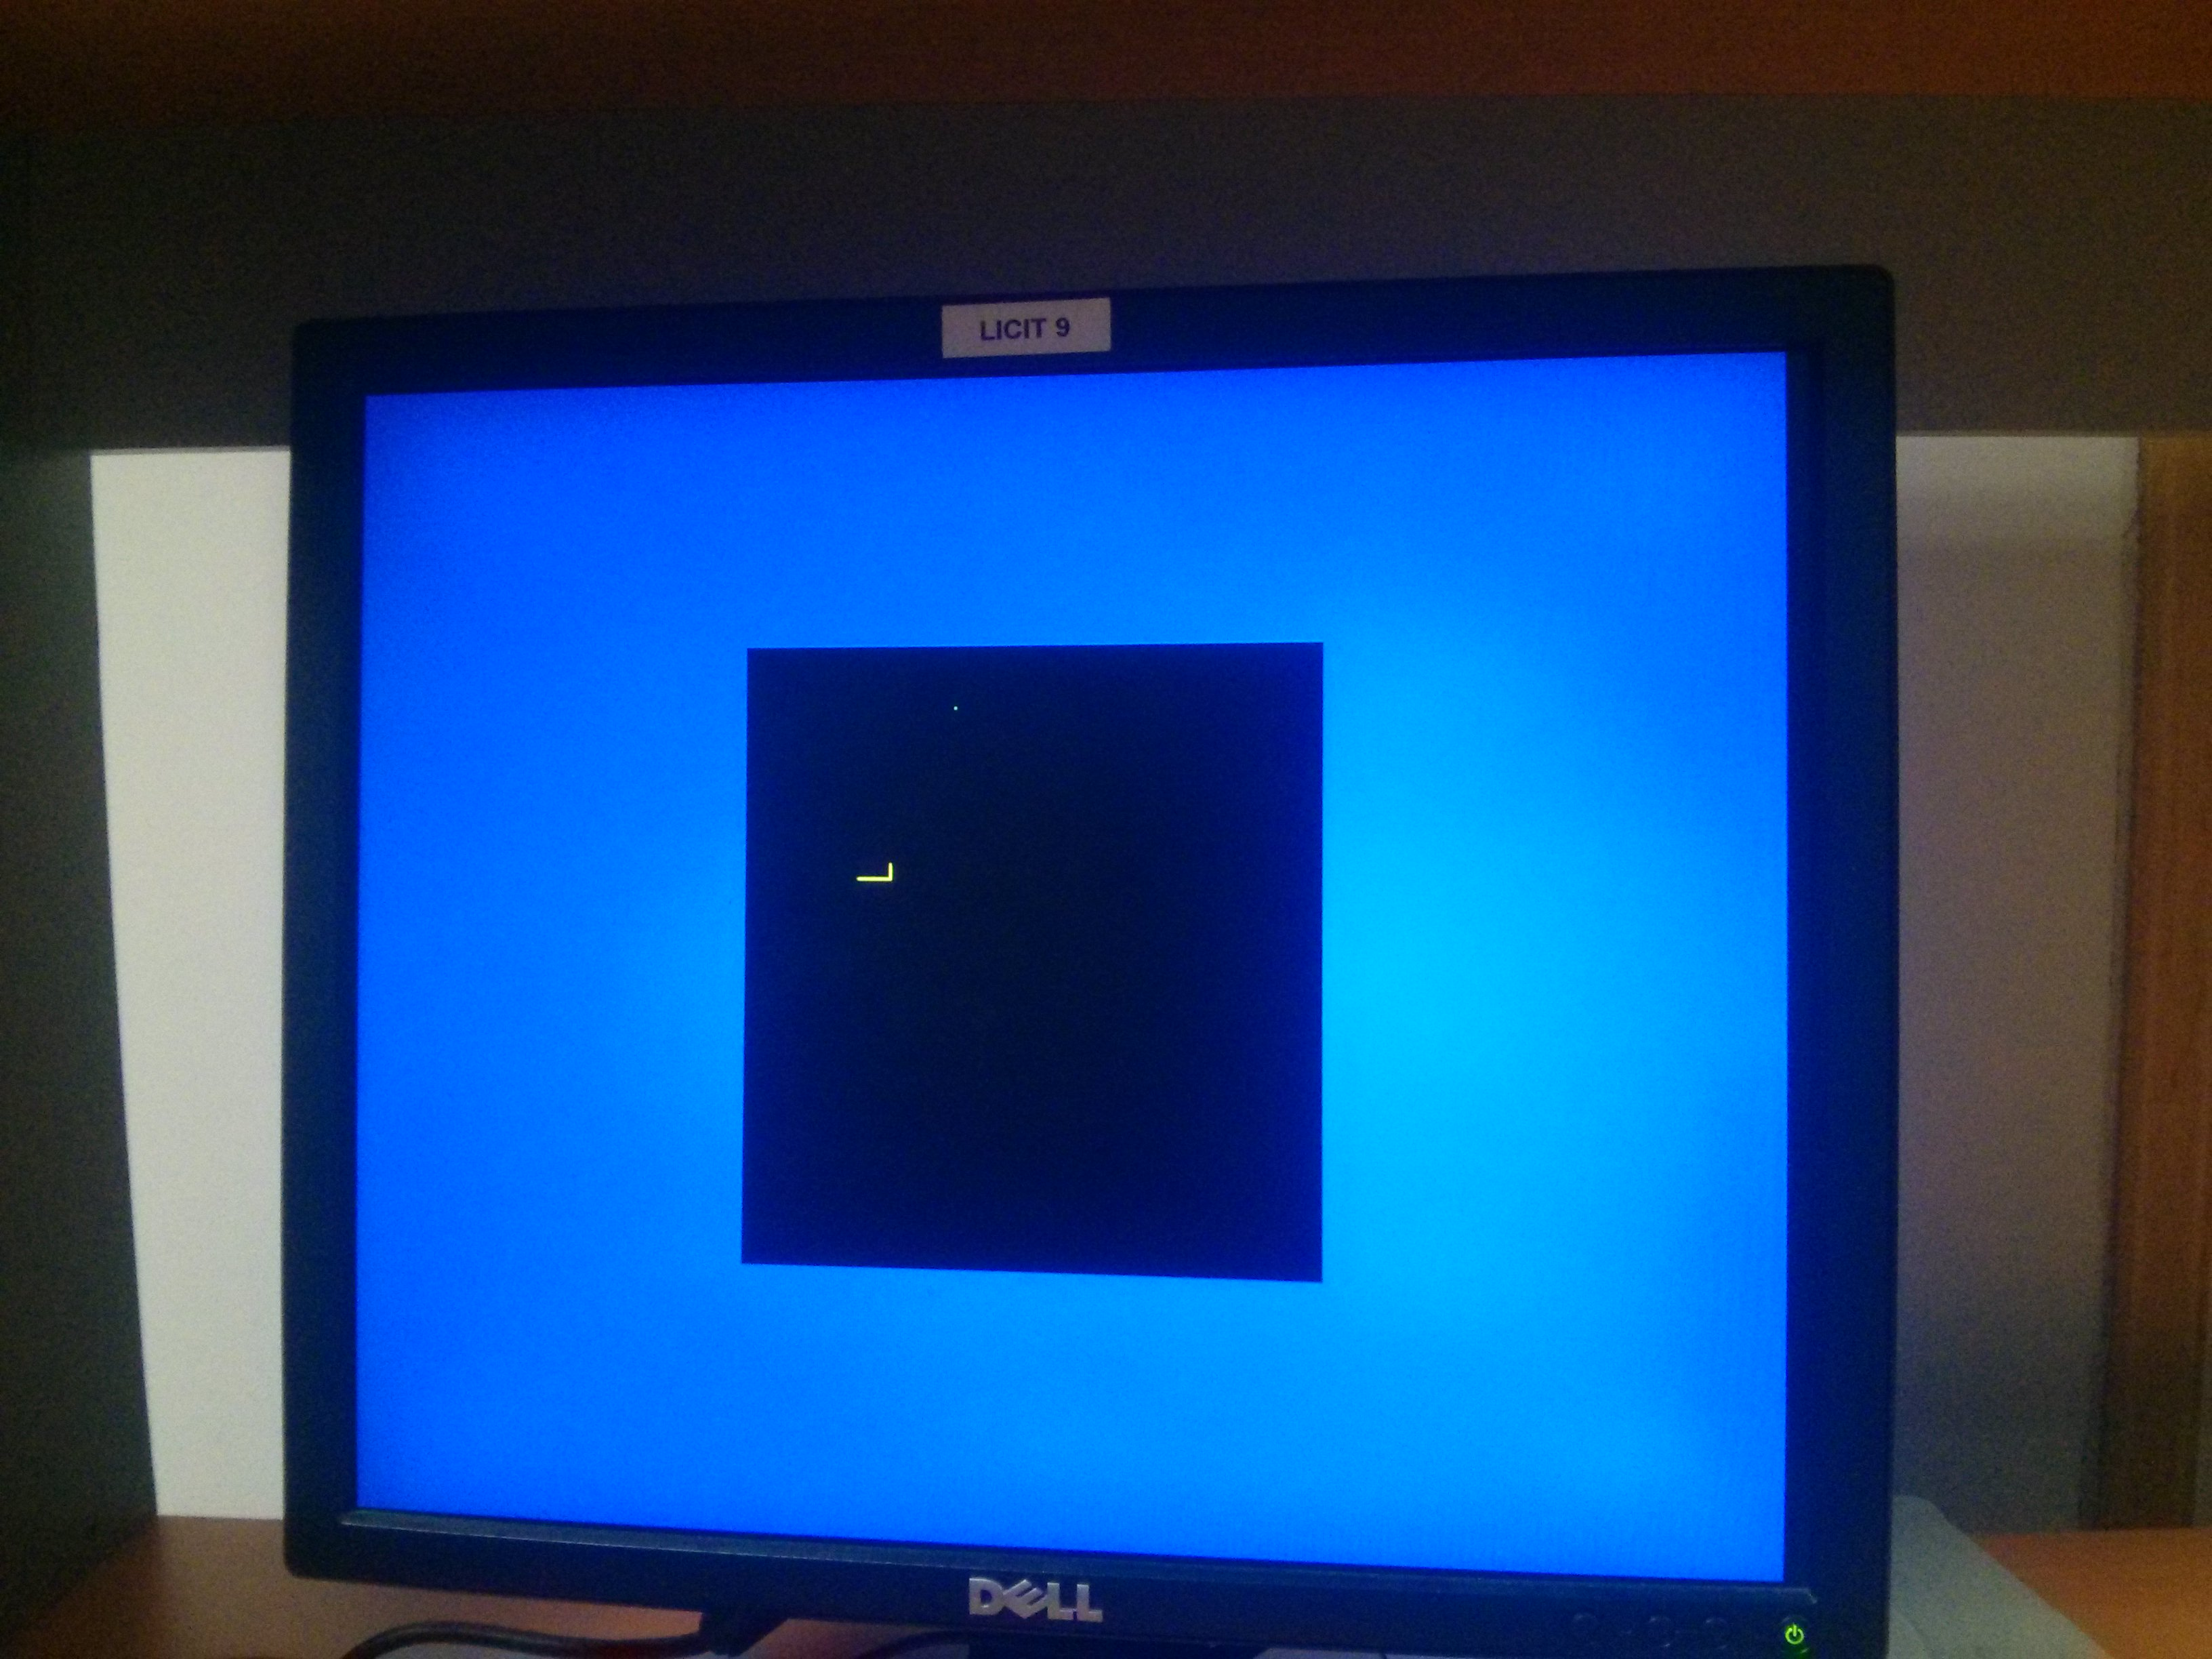
\includegraphics[width=1\textwidth]{game-play}
\caption{Game play}
\label{vga-play}
\end{figure}

\begin{figure}[hbtp]
\centering
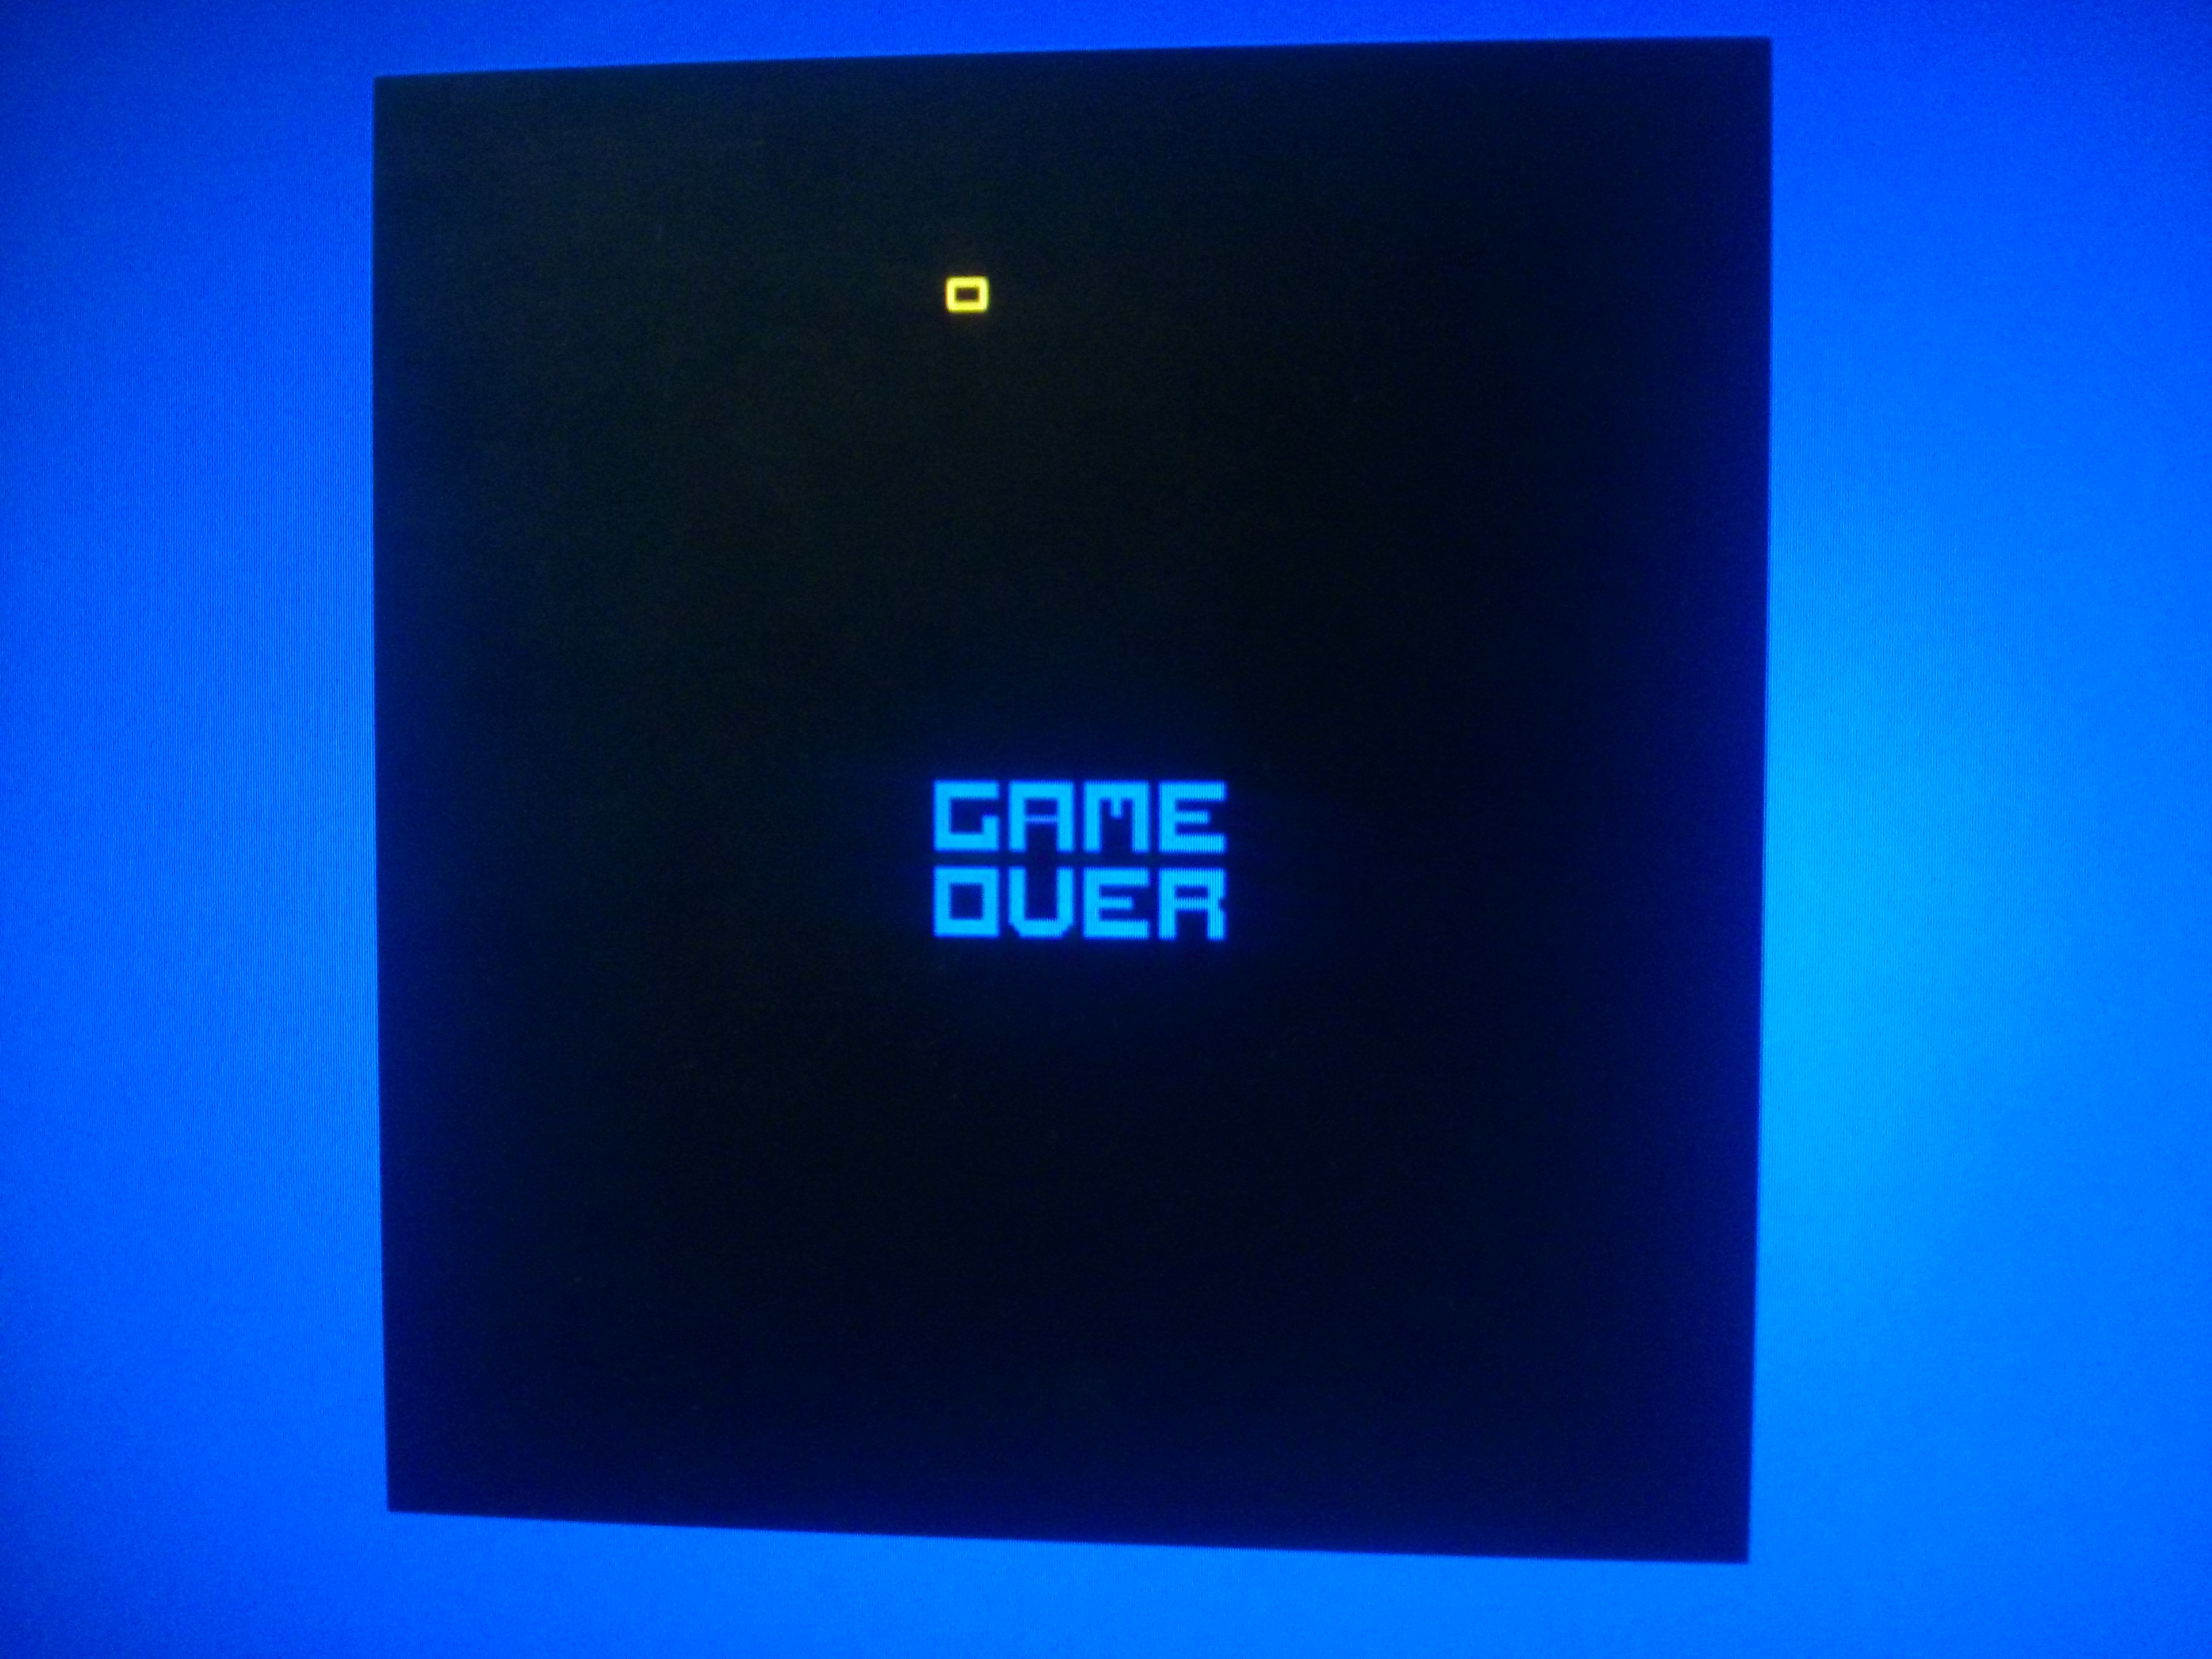
\includegraphics[width=1\textwidth]{game-over}
\caption{Game over tocandose así mismo}
\label{vga-over}
\end{figure}

\begin{figure}[hbtp]
\centering
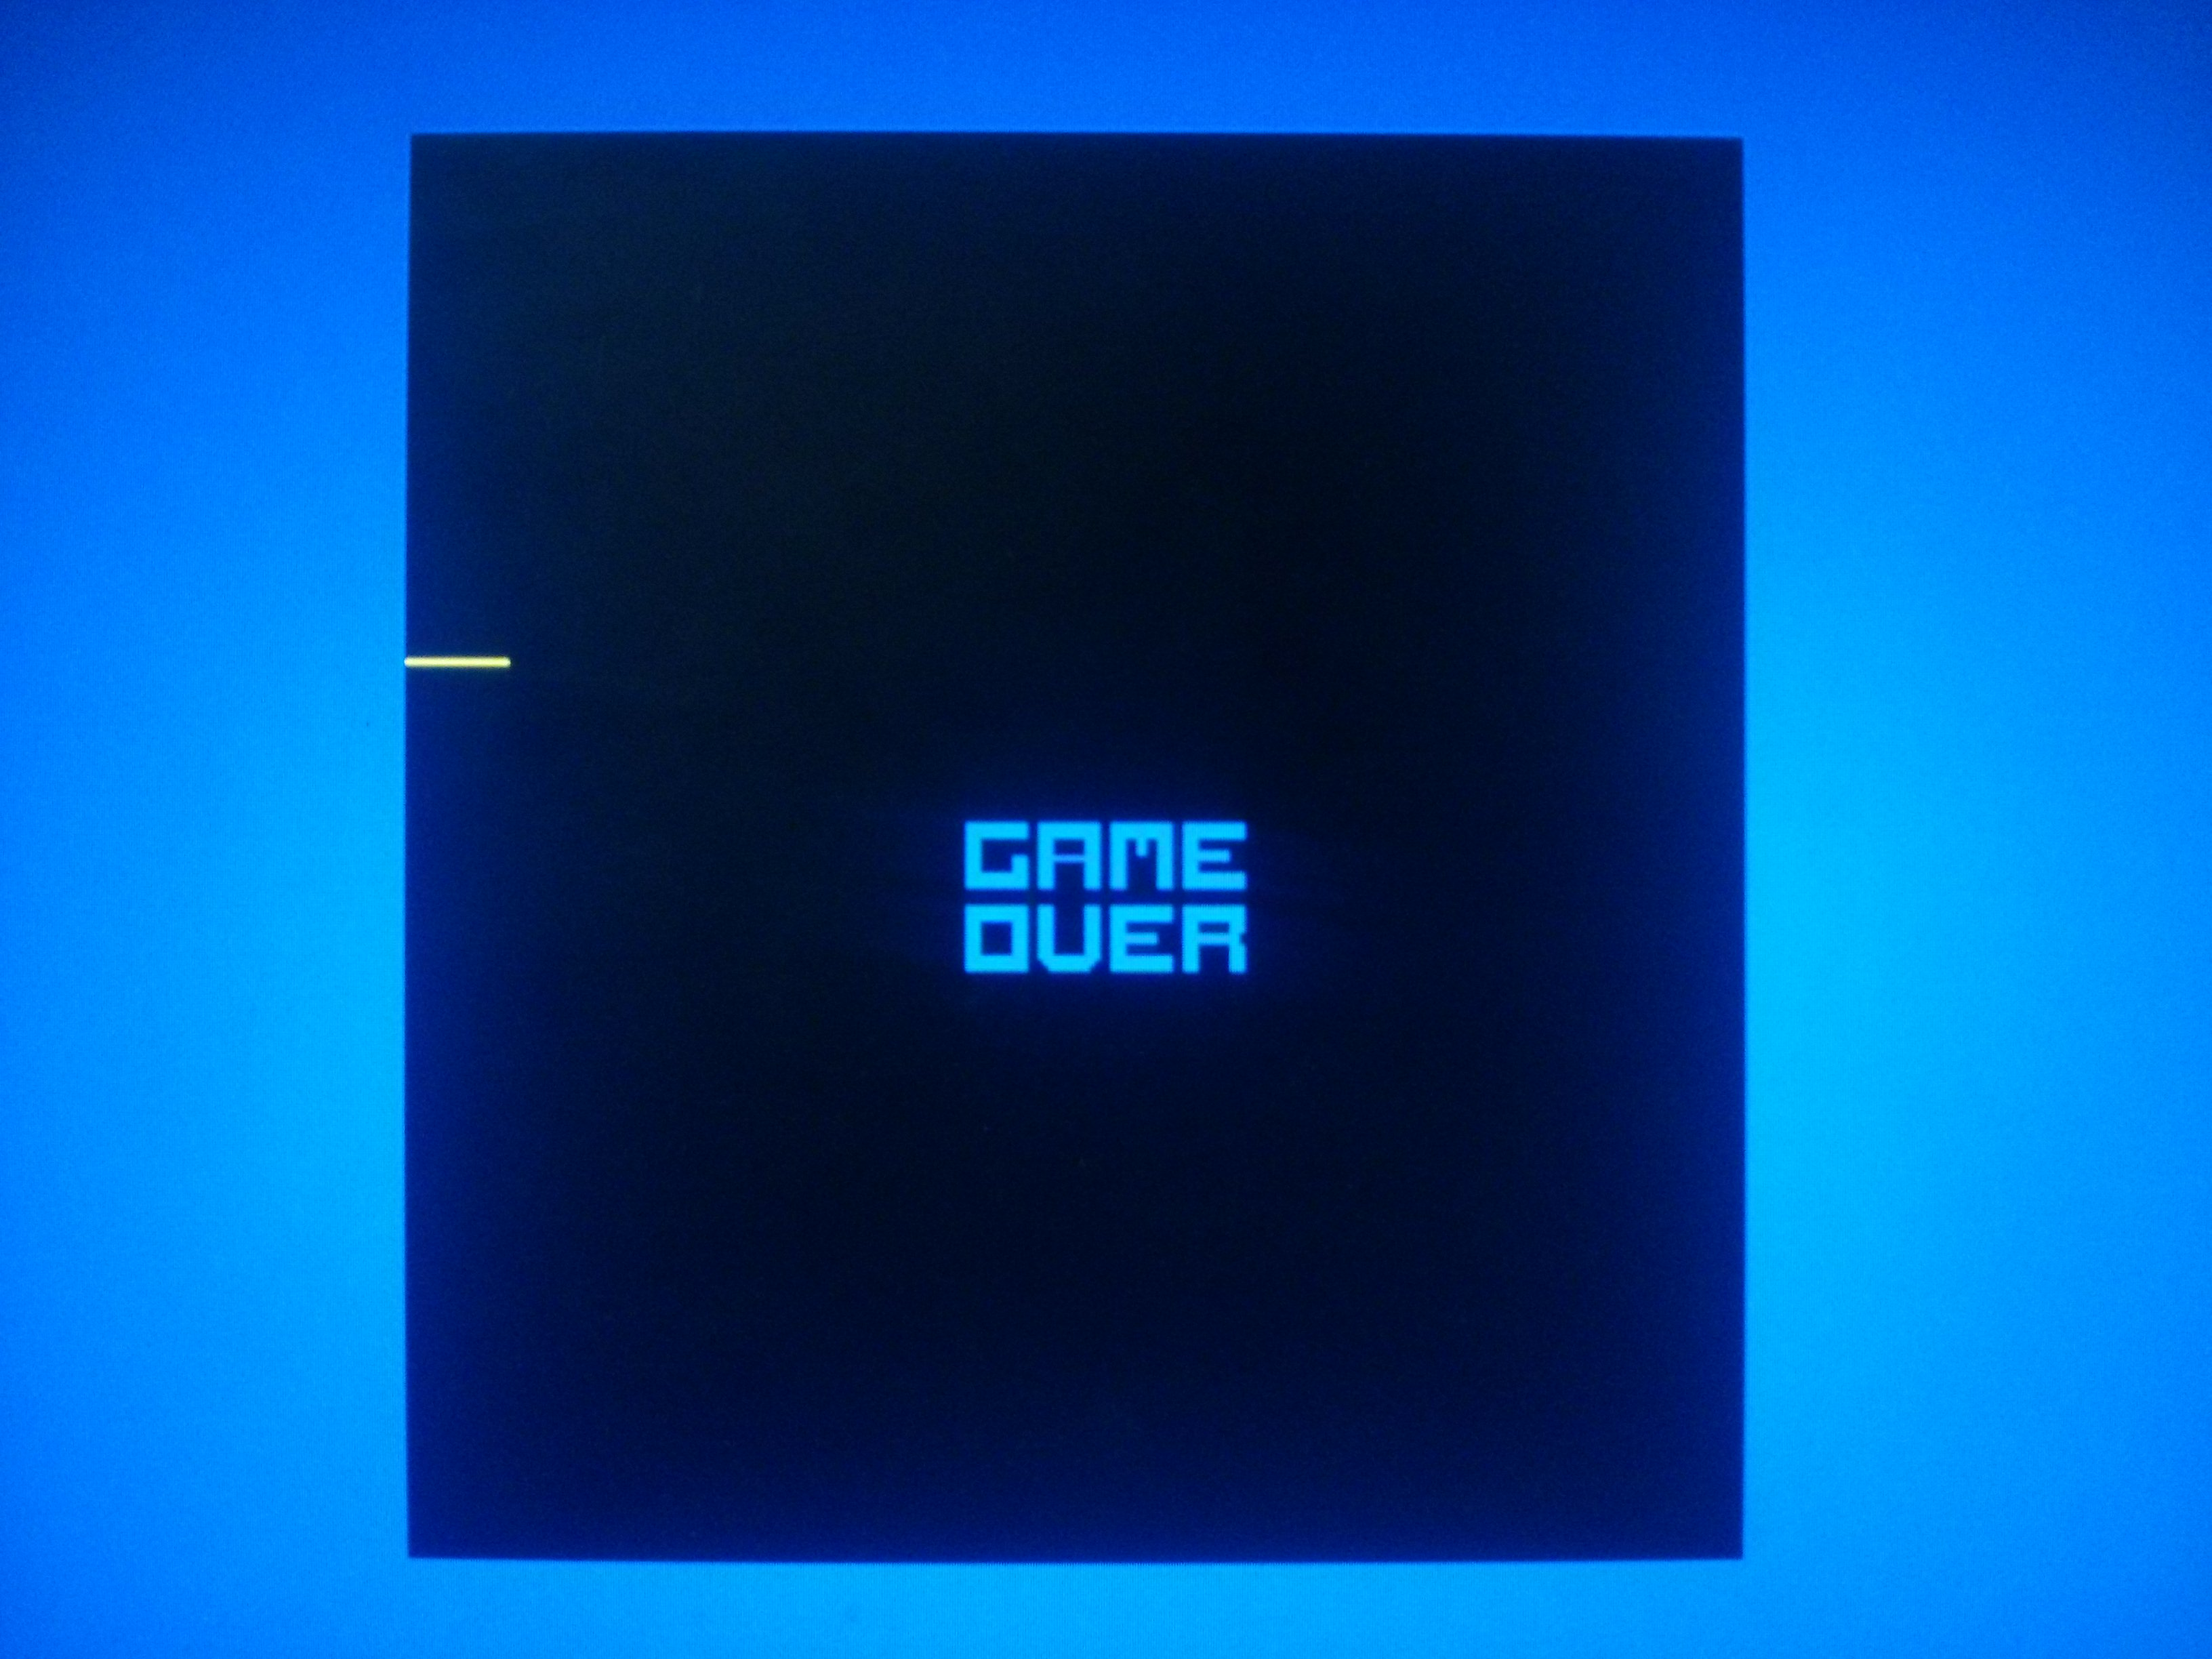
\includegraphics[width=1\textwidth]{game-over-side}
\caption{Game over tocando un lado}
\label{vga-over-side}
\end{figure}

%%**********************************************************************
\section{Discución}
Hablar de la comida que se salia del mapa
numero aleatorios
dificultad de hacer la serpiente mas grande (q agarre mas pixeles)
%%**********************************************************************
\section{Conlusiones}
recomendaciones
que se implemento y que no
%%**********************************************************************
\bibliography{bitacora}
\bibliographystyle{abbrv}
\end{document}
%%*************************************************************************
